\documentclass[tikz,border=10pt]{standalone}
% Scale s = 0.0181 cm per px (STYLE METRICS); y axis flipped
\begin{document}
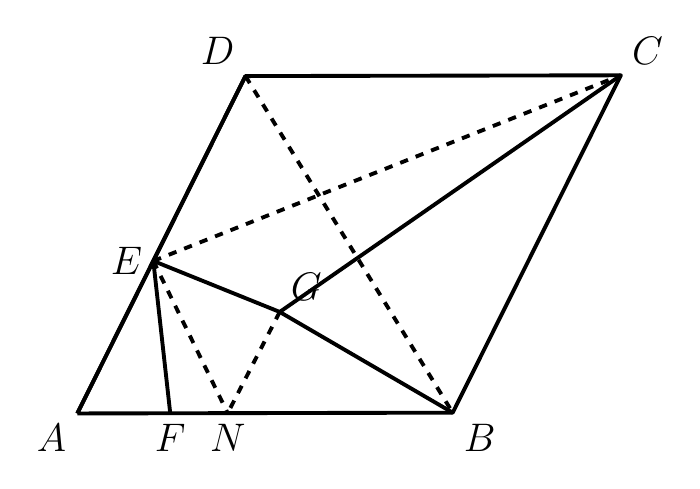
\begin{tikzpicture}[line join=round, line width=1.4pt,
  every node/.style={font=\fontsize{14.5}{17.4}\selectfont}]

% Named vertices (converted from pixel coordinates)
\coordinate (A) at (-3.480249116124663,-2.1390080428020894);
\coordinate (B) at (1.287385980310502,-2.1290089539456627);
\coordinate (C) at (3.4225816161634293,2.155753074830958);
\coordinate (D) at (-1.345053480271736,2.1457539859745305);
\coordinate (E) at (-2.5150609714132455,-0.2021356346525549);
\coordinate (F) at (-2.3001021529372396,-2.136532938455833);
\coordinate (G) at (-0.9094108694010374,-0.8498195938113808);
\coordinate (N) at (-1.5700910063260105,-2.1350018971379674);

% Solid outline
\draw (A) -- (B) -- (C) -- (D) -- (A);
% Solid: A--E--D lies on line AD
\draw (A) -- (D);
% Solid: E--F
\draw (E) -- (F);
% Solid: E--G--B (shallow bend at G is real)
\draw (E) -- (G) -- (B);
% Solid: C--G (restored, CV line_01 confirmed solid)
\draw (C) -- (G);

% Dashed edges
\draw[dashed] (E) -- (C);
\draw[dashed] (D) -- (B);
\draw[dashed] (E) -- (N);
\draw[dashed] (G) -- (N);

% Labels
\node[below left] at (A) {$A$};
\node[below right] at (B) {$B$};
\node[above right] at (C) {$C$};
\node[above left] at (D) {$D$};
\node[left] at (E) {$E$};
\node[below] at (F) {$F$};
\node[above right] at (G) {$G$};
\node[below] at (N) {$N$};

\end{tikzpicture}
\end{document}